\section{ \textbf{G}roup \textbf{P}articipation \textbf{I}mpact \textbf{T}ool (GPIT) and \textbf{G}roup \textbf{A}ctivity \textbf{I}mpact \textbf{T}ool (GAIT)}
\paragraph*{GAIT}~\\
The GAIT is used for monitoring the relative workload of all members of a team. This will assist in evenly distributing the workload, possibly increasing the overall productivity of the team. Additionally, the tool exposes any team members that are less productive than what is expected. Every task has to be manually weighted to reflect the difficulty and workload of the task. If the difficulty or workload of a task is under- or over-estimated the reflection of the workload of the members given by the tool will not be correct.
This tool has been used only sparingly throughout the course of the project. Very often it has been hard to identify individual tasks and harder still to determine the importance/weight of each task. These difficulties meant that any benefits of distributing tasks using the tool did not compensate for the extra time associated with using the tool. 
[Is the following reasonable?] By not using any structured method of distributing tasks, other than identifying tasks (where possible) and people voulenteering for any task that they find interesting, we may have skewed the relative workload of the members. Certainly, it has meant that some people have worked almost exclusively on one area within the project.
\begin{landscape}
	\begin{figure}[h!]
		\label{fig:GAIT}
		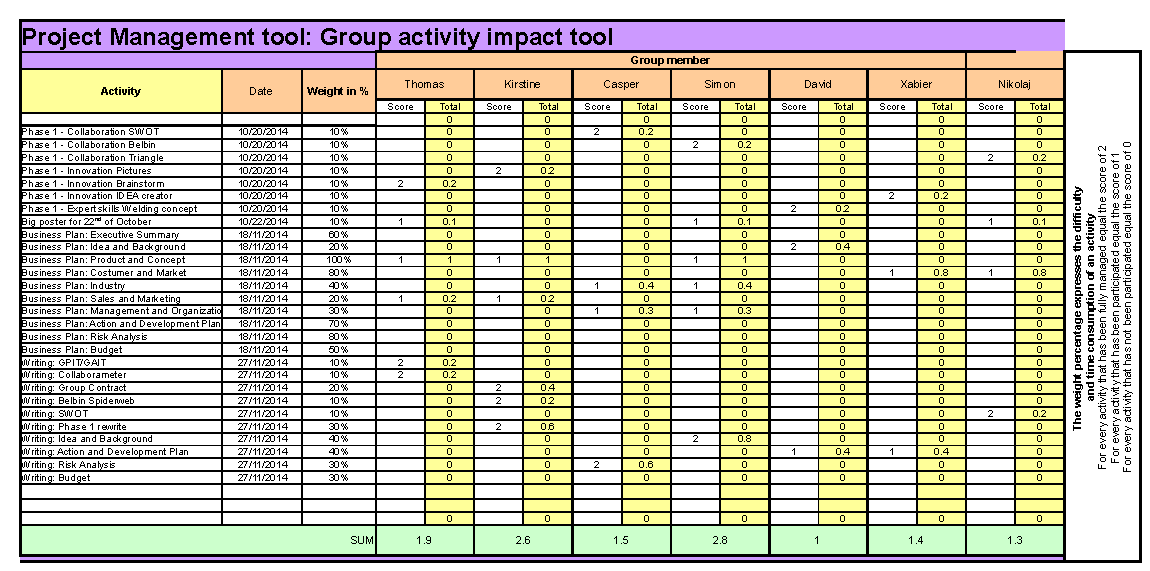
\includegraphics[scale=1.25]{./graphics/GAIT}
		\caption{The GAIT tool with all the entries made by the group}
	\end{figure}
\end{landscape}
\paragraph*{GPIT}~\\
The GPIT is simply a tool for monitoring the meeting participation of each individual member. It provides a graphical representation of the participation. Using this tool will provide the team with concrete evidence of the participation of each member. This could prove useful, should a situation where a team members contribution is in question arise. This tool was used throughout the first month of the project but was since neglected. The results can be seen in figures \ref{fig:GPIT} and \ref{fig:GPITGraph}. Since the GPIT has only been filled out the first month, obviously, it does not give a complete image of the participation. But since the group contract says that prople has to work eifht hours per week, and attend all group meetings, but not anythig about where these hours should be, not filling it out does not give any problems. When working this way keeping track of the GAIT is more important. 
\todo[inline]{Update GPIT picture with names.}
\begin{figure}[h!]

	\makebox[\textwidth][c]{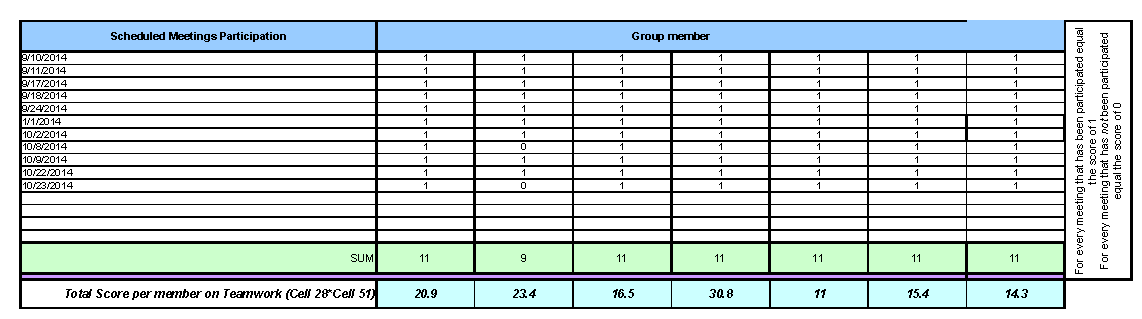
\includegraphics[scale=1]{./graphics/GPIT}}
	\caption{The GPIT tool with all the entries made by the group. If the person was there on the given date, they are given a 1, and if not, a 0. }
		\label{fig:GPIT}
\end{figure}

\begin{figure}[h!]

	\makebox[\textwidth][c]{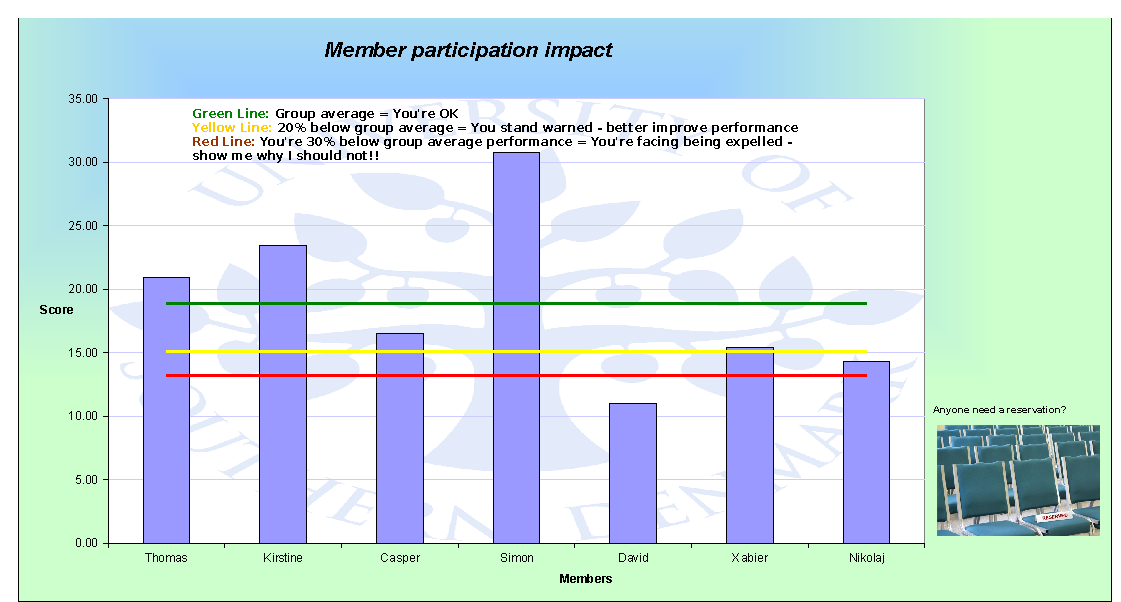
\includegraphics[scale=1]{./graphics/GPITGraph}}
	\caption{The GAIT tool with all the entries made by the group}
	\label{fig:GPITGraph}	
\end{figure}